\documentclass[a4paper,11pt]{article}
%\usepackage{isolatin1}
%\usepackage{german}
\usepackage{float}
\usepackage{listings}
\usepackage{graphicx}
\usepackage{lastpage}
\usepackage{fancyhdr}
\usepackage{soul}
\usepackage{array}
\usepackage{amssymb}
\usepackage{wrapfig}

\usepackage{lmodern} % Latin Modern

\usepackage[ngerman]{babel, translator}
\usepackage[utf8]{inputenc}
\usepackage[hyphens]{url}

%\usepackage[utf8x]{inputenc}
\usepackage[left=2.5cm,top=2cm,right=2cm,bottom=4cm]{geometry}

%Code listings
\usepackage{listingsutf8}


%\usepackage[]{hyperref}
%\hypersetup{
%	linkcolor=blue, 
%	pagecolor= blue,
%	urlcolor= blue,
%	colorlinks=true,
%	pdfborder=0 0 0
%}
\usepackage[
nonumberlist, %keine Seitenzahlen anzeigen
acronym,      %ein Abk�rzungsverzeichnis erstellen
toc,          %Eintr�ge im Inhaltsverzeichnis
section]      %im Inhaltsverzeichnis auf section-Ebene erscheinen
{glossaries}


%\usepackage{hyperref}

%Ein eigenes Symbolverzeichnis erstellen
\newglossary[slg]{symbolslist}{syi}{syg}{Symbolverzeichnis}

%Den Punkt am Ende jeder Beschreibung deaktivieren
\renewcommand*{\glspostdescription}{}

%Glossar-Befehle anschalten
\makeglossaries

%Diese Befehle sortieren die Eintr�ge in den
%einzelnen Listen:
%makeindex -s datei.ist -t datei.alg -o datei.acr datei.acn
%makeindex -s datei.ist -t datei.glg -o datei.gls datei.glo
%makeindex -s datei.ist -t datei.slg -o datei.syi datei.syg



%Befehle f�r Abk�rzungen
\newacronym{BDD}{BDD}{Behaviour Driven Development}

%Befehle f�r Glossar


\renewcommand{\familydefault}{\sfdefault}


%Einstellungen f??r code listings
\lstset{inputencoding=latin1, language=Java,tabsize=2, basicstyle=\small,breaklines=true,showstringspaces=false}
\pagestyle{fancy}
\setlength{\headwidth}{470pt}
\renewcommand{\headrule}{\hskip -\leftskip{\bf \quad \quad}\vbox to 5pt{\hbox to 455pt{\hrulefill}}}
\renewcommand{\footrule}{\hskip-\leftskip{\bf \quad \quad}{\hbox to 450 pt{\hrulefill}\newline}}
\fancyhf{}
\fancyheadoffset[L]{1cm}
\fancyfootoffset[L]{1cm}
%Kopfzeile links bzw. innen
\fancyhead[L]{
\includegraphics[height=0.5in]{img/fhnw_ht_10mm.jpg}}
%Kopfzeile mittig
\fancyhead[C]{}
%Kopfzeile rechts bzw. au??????????�?en
\fancyhead[R]{\hspace{10pt} \\MVDBS Lab\\ \rightmark }
  \fancyheadoffset[L]{1cm}
  \fancyfootoffset[L]{1cm}
%Linie oben
\renewcommand{\headrulewidth}{0.7pt}
%Fu??????????�?zeile mittig
\cfoot{Seite:\ \thepage\ von \pageref{LastPage}}
\fancyfoot[R]{}

\usepackage{color}
\usepackage{xcolor}
\usepackage{listings}
\usepackage{caption}
\DeclareCaptionFont{white}{\color{black}}
\DeclareCaptionFormat{listing}{\colorbox{white}{\parbox{\textwidth}{#1#2#3}}}
\captionsetup[lstlisting]{format=listing,labelfont=white,textfont=white,font=bf}


\lstdefinestyle{sqlNoTitle}{
   language=SQL,
   basicstyle=\footnotesize\ttfamily, % Standardschrift
   backgroundcolor=\color[RGB]{230,230,230}, % Hintergrundfarbe
   numbers=left,               % Ort der Zeilennummern
   numberstyle=\tiny,          % Stil der Zeilennummern
   stepnumber=1,               % Abstand zwischen den Zeilennummern
   numbersep=5pt,              % Abstand der Nummern zum Text
   tabsize=2,                  % Groesse von Tabs
   extendedchars=true,         % Erlaubt non-ascii Charakter, aber nicht mit UTF8
   literate={ä}{{\"a}}1 {ü}{{\"u}}1 {ö}{{\"o}}1,
   breaklines=true,            % Zeilen werden Umgebrochen
   frame=trbl,                 % Rahmen
   stringstyle=\color[RGB]{42,0,255} \ttfamily, % Farbe der String
   keywordstyle=\color[RGB]{127,0,85} \ttfamily, % Farbe der Keywords
   commentstyle=\color[RGB]{63,127,95} \ttfamily, % Farbe des Kommentars
   showspaces=false,           % Leerzeichen anzeigen ?
   showtabs=false,             % Tabs anzeigen ?
   xleftmargin=17pt,
   framexleftmargin=17pt,
   framexrightmargin=5pt,
   framexbottommargin=5pt,
   framextopmargin=5pt,
   showstringspaces=false,     % Leerzeichen in Strings anzeigen ?
}


\lstdefinestyle{sql}{
   style=sqlNoTitle,
   title=SQL-Skript
}

\lstdefinestyle{queryResult}{
  basicstyle=\footnotesize\ttfamily, % Standardschrift
  backgroundcolor=\color[RGB]{240,255,240}, % Hintergrundfarbe
  frame=trbl,                 % Rahmen
  literate={ä}{{\"a}}1 {ü}{{\"u}}1 {ö}{{\"o}}1,
}

\lstdefinestyle{queryResultSmall}{
  style=queryResult,
  basicstyle=\scriptsize\ttfamily, % Standardschrift
}

%Linie unten
\renewcommand{\footrulewidth}{0.5pt}

\vspace*{15mm}
\textwidth 450pt



\begin{document}

\setcounter{tocdepth}{5}



%\thispagestyle{empty}

\begin{center}

\vspace{48pt}


\begin{Huge}
\noindent {Mobile und Verteilte Datenbank Systeme - Zusammenfassung}
\end{Huge}\\ 
\vspace{10pt}
\begin{center}
\begin{Large}
Egemen Kaba
\end{Large}
\end{center}

\vspace{10pt}



\end{center}

\newpage


\newpage

\tableofcontents

%Glossar ausgeben
%Glossar ausgeben


\vspace{12pt}


\newpage
\section{Kapitel 0 - Introduction}
\begin{tabular}{| p{5cm} | p{10cm} |}
\hline
Verteilte Datenbank (DDB) & Eine verteilte Datenbank ist eine Sammlung mehrerer, untereinander logisch zusammengehöriger Datenbanken, die über ein Computernetzwerk verteilt sind.\\ \hline
Verteiltes Datenbankverwaltungssystem (D-DBMS) & Ein verteiltes Datenbankverwaltungssystem ist die Software, die die verteilte Datenbank verwaltet und gegenüber den Nutzern einen transparenten Zugang erbringt.\\ \hline
Verteiltes Datenbank System (DDBS) & DDBS = DBS + D-DBMS\\ \hline
Nebenläufigkeit & 
\begin{itemize}
\item Synchronisation konkurrierender Transaktionen
\item Konsistenz und Isolation
\item Deadlock Erkennung
\end{itemize}\\ \hline
Zuverlässigkeit &
\begin{itemize}
\item Robustheit gegenüber Fehler
\item Atomarität und Dauerhaftigkeit
\end{itemize}\\ \hline
Architekturen &
\begin{itemize}
\item Shared Memory Architecture
\item Shared Disk Architecture
\item Shared Nothing Architecture
\end{itemize}\\ \hline
Mobile Datenbank Systeme & 
Verteilte Datenbank System mit zusätzlichen Eigenschaften und Einschränkungen
\begin{itemize}
\item beschränkte Ressource
\item häufig nicht verbunden
\item verlangt andere Transaktions Modelle
\item verlangt andere Replikationsstrategien
\item Ortsabhängigkeit
\end{itemize}\\ \hline
\end{tabular}\\
\\
\textbf{Date's 12 Regeln}
\begin{itemize}
\item Lokale Autonomie
\item Unabhängigkeit von zentralen Systemfunktionen
\item Hohe Verfügbarkeit
\item Ortstransparenz
\item Fragmentierungstransparenz
\item Replikationstransparenz
\item Verteilte Anfragebearbeitung
\item Verteilte Transaktionsverarbeitung
\item Hardware Unabhängigkeit
\item Betriebssystem Unabhängigkeit
\item Netzwerkunabhängigkeit
\item Datenbanksystem Unabhängigkeit
\end{itemize}
\section{Kapitel 1 - Trigger}
\subsection{Zweck}
\begin{itemize}
\item Realisieren aktive Datenbanksysteme
\item Berechnung abgeleiteter Attribute
\item Überprüfen komplexer Integritätsbedingungen
\item Implementierung von Geschäftsregeln
\item Protokollierung, Statistiken
\item Überprüfen von Integritätsbedingungen in verteilten Datenbanken
\item Synchronisation von Replikaten
\end{itemize}
\subsection{Konzepte}
\begin{tabular}{| p{5cm} | p{10cm} |}
\hline
ECA Prinzip &
Event: Ereignis tritt ein\newline
Condition : Bedingung ist erfüllt\newline
Action: Aktion wird ausgeführt\\ \hline
Ereignis &
DML: UPDATE, DELETE, INSERT\newline
DDL: CREATE, ALTER, DROP, ...\newline
Datenbank: SERVERERROR, LOGON, LOGOFF, STARTUP, SHUTDOWN\newline
(DML-Trigger können auf Tabellen oder Views definiert werden)\\ \hline
Timing & BEFORE, AFTER, INSTEAD OF Trigger\newline
Der INSTEAD OF Trigger ersetzt den triggernden Befehl und wird nur bei Views eingesetzt.\\ \hline
Granulat & STATEMENT, ROW Trigger\\ \hline
\end{tabular}
\subsection{Struktur eines Triggers}
\begin{lstlisting}[style=sql, title=Syntax]
CREATE [OR REPLACE] TRIGGER tname
{BEFORE|AFTER} events
[WHEN(condition)]
pl/sql_block
\end{lstlisting}
\begin{lstlisting}[style=sql, title=events]
{DELETE|INSERT|UPDATE
	[OF column [ , column ]...] }
[OR {DELETE|INSERT|UPDATE
	[OF column [ , column ]...]}]...
ON table [FOR EACH ROW]
\end{lstlisting}
\begin{lstlisting}[style=sql, title=Prinzip]
DECLARE
	Deklarationsteil
BEGIN
	Programmteil
EXCEPTION
	Ausnahmebehandlung
END;
/
\end{lstlisting}
\begin{lstlisting}[style=sql, title=Bildschirmausgabe]
dbms_output.put_line (item IN VARCHAR2);
dbms_output.put_line (item IN NUMBER);
dbms_output.put_line (item IN DATE);
dbms_output.put(item IN VARCHAR2);
dbms_output.put(item IN NUMBER);
dbms_output.put(item IN DATE);
dbms_output.new_line;
-- Ausführung
EXECUTE dbms_output.put_line('Hello world');
-- als Block
BEGIN
	dbms_output.put_line('Hello world');
END;
\end{lstlisting}
\textbf{Datentypen}\\
\begin{itemize}
\item SQL: VARCHAR2, DATE, NUMBER, ...
\item PL/SQL: BOOLEAN, PLS\_INTEGER, ...
\item Strukturierte Datentypen: TABLE, VARRAY, RECORD
\item Datentypen für Spalten und Zeilen aus Tabellen: \% ROWTYPE, \%TYPE
\end{itemize}
\begin{lstlisting}[style=sql, title=Zuweisung]
-- Syntax
variable := expression;
-- Beispiel im Deklarationsteil
name VARCHAR2(30) := 'Kaba';
\end{lstlisting}
\begin{lstlisting}[style=sql, title=if then else elsif]
IF condition THEN ... END IF;
IF condition THEN ... ELSIF condition THEN ... ELSE ... END IF;
IF condition THEN ... ELSE ... END IF;
\end{lstlisting}
\begin{lstlisting}[style=sql, title=if then else elsif]
IF condition THEN ... END IF;
IF condition THEN ... ELSIF condition THEN ... ELSE ... END IF;
IF condition THEN ... ELSE ... END IF;
\end{lstlisting}
\begin{lstlisting}[style=sql, title=schleifen]
WHILE condition LOOP ... END LOOP;
FOR counter IN lower_bound..higher_bound LOOP ... END LOOP;
\end{lstlisting}
\subsection{Beispiel}
\begin{lstlisting}[style=sql, title=Trigger]
CREATE OR REPLACE TRIGGER regdatum_test
	BEFORE INSERT ON registrierungen
	FOR EACH ROW
	
	DECLARE
		msg VARCHAR2(30) := 'Datum falsch';
	BEGIN
		IF :new.datum > SYSDATE THEN
			RAISE_APPLICATION_ERROR(-20005, msg);
		END IF;
END;
\end{lstlisting}
\subsection{Databaselinks}
Datenbanklinks werden benötigt, um Orts- und Namenstransparenz für Tabellen zu erreichen.
\begin{lstlisting}[style=sql, title=Databaselinks]
-- View
CREATE OR REPLACE VIEW filme AS
SELECT *
FROM filme@ananke.hades.fhnw.ch;
-- Synonyme
CREATE SYNONYM film FOR filme@ananke.hades.fhnw.ch;
\end{lstlisting}
\section{Kapitel 2 - Distributed Design I}
Ausgangslage: Anwendungen auf verschiedenen Knoten des Netzwerks greifen auf eine (relationale) Datenbank zu. Nun greifen nicht alle Knoten gleich häufig auf den selben Datensatz zu. Es gilt nun herauszufinden, welche Anwendungen (Queries) auf welchen Knoten welche Daten mit welcher Häufigkeit benötigen. Das Resultat ist eine Menge von Fragmenten, die den verschiedenen Knoten zugeteilt werden.
\subsection{Arten der Fragmentierung}
\begin{itemize}
\item Horizontale Fragmentierung (HF) (Abbildung \ref{fig:horizontalFrag})
\begin{itemize}
\item Primäre horizontale Fragmentierung (PHF)
\item Abgeleitete horizontale Fragmentierung (DHF)
\end{itemize}
\item Vertikale Fragmentierung (VF) (Abbildung \ref{fig:verticalFrag})
\item Gemischte Fragmentierung (MF)
\end{itemize}
\begin{figure}[ht]
  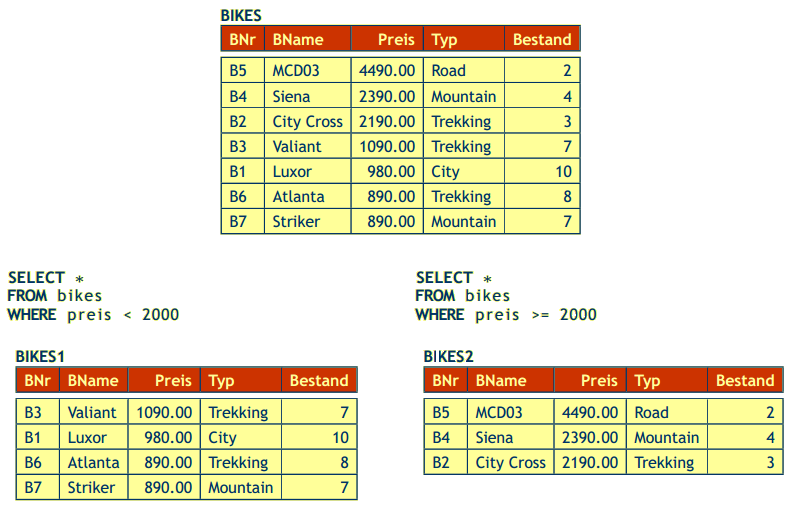
\includegraphics[scale=0.75]{src/horizontale_fragmentierung.png}
	\caption{Horizontale Fragmentierung}
	\label{fig:horizontalFrag}
\end{figure}
\begin{figure}[ht]
  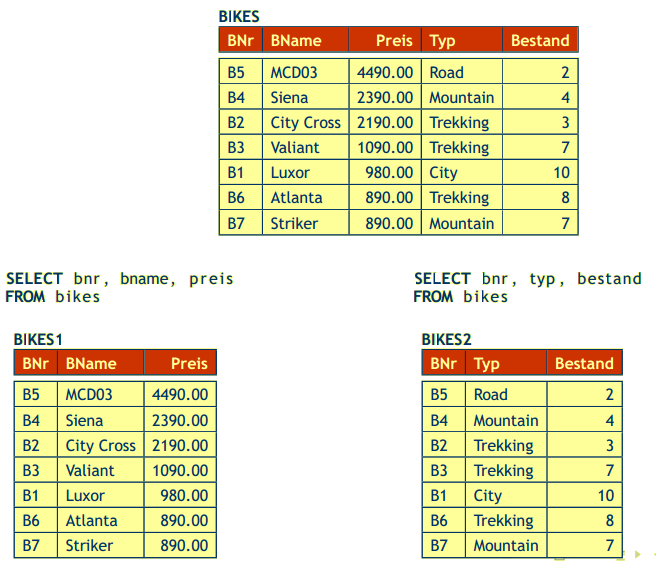
\includegraphics[scale=0.75]{src/vertikale_fragmentierung.png}
	\caption{Vertikale Fragmentierung}
	\label{fig:verticalFrag}
\end{figure}
\subsection{PHF}
\subsubsection{Predicates}
\begin{tabular}{| p{5cm} | p{5cm} | p{6cm} |}
\hline 
Simple predicates & Vergleich eines Attributs mit einem Wert (WHERE-Klausel) & \begin{center}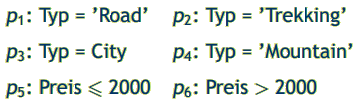
\includegraphics[scale=0.5]{src/simple_predicates.png}\end{center}\\ \hline
Minterm predicates & Verknüpfung von Simple predicates mit AND und NOT & \begin{center}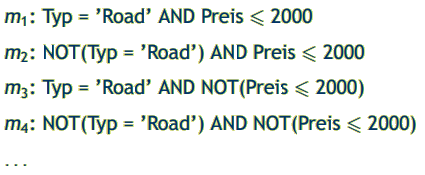
\includegraphics[scale=0.5]{src/minterm_predicates.png}\end{center}\\ \hline
Vollständigkeit & \multicolumn{2}{p{10cm}|}{Eine Menge von simple predicates ist vollständig genau dann, wenn au fbeliebige 2 Tupel im gleichen Fragment von allen Anwendungen mit der gleichen Häufigkeit zugegriffen wird}\\ \hline
Minimalität & \multicolumn{2}{p{10cm}|}{Wird durch ein simple predicate ein Fragment weiter aufgeteilt, dann muss es mindestens eine Anwendung geben, die auf diese Fragmente verschieden zugreift. Ein simple predicate soll also relevant sein für die Bestimmung einer Fragmentierung. Sind alle simple predicate einer Menge P relevant, dann ist P minimal}\\ \hline
\end{tabular}
\subsubsection{PHF Beispiel}
\begin{tabular}{| p{3cm} | p{5cm} | p{4cm} | p{4cm}|}
\hline
Anwendung & Query & Parameter & Simple Predicates \\ \hline
Anwendung 1 & SELECT bname, bestand \newline FROM bikes \newline WHERE typ = ? & 
City (4/Woche) \newline
Trekking (3/Woche) \newline
Mountain (2/Woche) \newline
Road (1/Woche) & 
p1: Typ = 'Road' \newline
p2: Typ = 'Mountain' \newline
p3: Typ = 'Trekking' \newline
p4: Typ = 'City'
\\ \hline
Anwendung 2 & SELECT * \newline FROM bikes \newline WHERE preis = ? &
$<$2000 (3/Woche) \newline
$>=$2000 (1/Woche) \newline &
p5: Preis $<$ 2000 \newline
p6: Preis $>=$ 2000
\\ \hline
\end{tabular}
Sinnvolle minterm predicates bilden. Zum Beispiel: m1: Typ = 'Road' AND Preis $<$ 2000.\\
\subsection{DHF}
Horizontale Fragmentierung auf einer übergeordneten horizontal fragmentierten Relation. Dadurch soll sichergestellt werden, dass auf häufig im Verbund zugegriffene Relationen auf dem selben Knoten liegen.\\
Falls die Tabelle KUNDEN nun in KUNDEN1 - KUNDEN4 fragmentiert werden, sieht die Fragmentierung der Tabele AUFTRAEGE wie folgt aus: AUFTRAEGEi = (AUFTRAEGE) $\ltimes$ (KUNDENi)
\section{Kapitel 3 - Distributed Design II}
\subsection{VF}
\subsubsection{Anwendungen als Queries}
\begin{tabular}{p{5cm}  p{5cm}}
q1 & q1\\ \hline
SELECT bestand\newline FROM bikes WHERE bname = ? & SELECT bestand, preis\newline FROM bikes\\ \\
q3 & q4\\ \hline
SELECT preis\newline FROM bikes WHERE typ = ? & SELECT AVG(bestand)\newline FROM bikes WHERE typ = ?
\end{tabular}
\subsubsection{[U]sage Matrix}
\begin{tabular}{|l||c|c|c|c|}
\hline
&BName&Preis&Typ&Bestand\\ \hline
q1 & 1 & 0 & 0 & 1 \\ \hline
q2 & 0 & 1 & 0 & 1 \\ \hline
q3 & 0 & 1 & 1 & 0 \\ \hline
q4 & 0 & 0 & 1 & 1 \\ \hline
\end{tabular}\\
1 = Query verwendet Attribut\\
0 = Query verwendet Attribut nicht
\subsubsection{[Acc]ess frequency Matrix}
\begin{tabular}{|c||c|c|c|}
&S1&S2&S3\\ \hline
q1 & 15 & 20 & 10\\ \hline
q2 & 5 & 0 & 0\\ \hline
q3 & 25 & 25 & 25\\ \hline
q4 & 3 & 0 & 0\\ \hline
\end{tabular}\\
Frage: Wie viel mal wird ein Query auf einem Knoten ausgeführt?\\
Da jetzt jedes Attribut ein Fragment bilden würde, muss jetzt nach einer Attributsmenge gesucht werden, auf die ähnlich zugegriffen wird.
\subsubsection{Affinitätsmatrix AA}
\begin{tabular}{|l||c|c|c|c|}
\hline
&BName&Preis&Typ&Bestand\\ \hline
BName & 45 & 0 & 0 & 45 \\ \hline
Preis & 0 & 80 & 75 & 5 \\ \hline
Typ & 0 & 75 & 78 & 3 \\ \hline
Bestand & 45 & 5 & 3 & 53 \\ \hline
\end{tabular}\\
Vorgehen: In der Access frequency Matrix Summer über jedes Query bilden (z.B. q1 = 45). Funktion aff(Ai,Aj) bestimmen durch Folgendes:
\begin{itemize}
\item Zeilen/Queries in der Usage Matrix suchen, die in diesen beiden Spalten eine 1 stehen haben.
\item Summen dieser Queries aus der Access frequency Matrix zusammenzählen.
\item In die Affinitätsmatrix in der Zeile/Spalte Ai und der Spalte/Zeile Aj eintragen.
\end{itemize}
\subsubsection{Bond Energy Algorithmus (BEA)}
Dieser Algorithmus maximiert die globale Affinität einer Affinitätsmatrix.\\
Die globale Affinität einer Matrix zu berechnen, muss die Funktion bond(Ax,Ay) für alle benachbarten Attribute ausgeführt werden.\\
Vorgehen Funktion bond(Ax,Ay):
\begin{itemize}
\item Über sämtliche Zeilen iterieren
\item Für jede Zeile den Eintrag in der Spalte Ax mit dem Eintrag in der Spalte Ay multiplizieren
\item Summe über diese Werte bilden
\end{itemize}
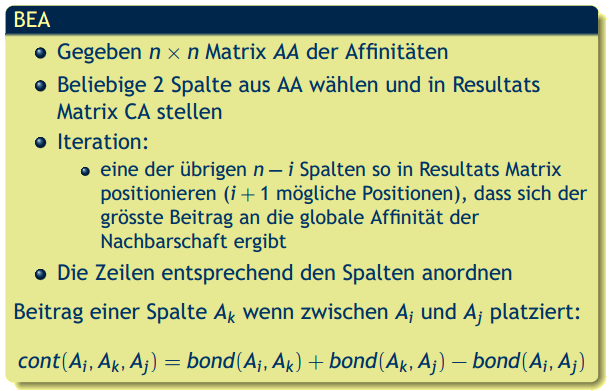
\includegraphics[scale=0.8]{src/bea.png}
\subsubsection{Splitting der Resultatsmatrix BEA}
\begin{tabular}{|l||c|c|c|c|}
\hline
&Bname&Bestand&Preis&Typ\\ \hline
BName & 45 & 45 & 0 & 0 \\ \hline
Bestand & 45 & 53 & 5 & 3 \\ \hline
Preis & 0 & 5 & 80 & 75 \\ \hline
Typ & 0 & 3 & 75 & 78 \\ \hline
\end{tabular}
Splitting mit Trennpunkt entlang der Diagonale führt zu drei Varianten:\\
\begin{itemize}
\item VF1: BName; VF2: Bestand,Preis,Typ
\item VF1: BName,Bestand; VF2: Preis,Type
\item VF1: BName,Bestand,Preis VF2: Typ
\end{itemize}
Die Variante mit der höchsten Trennqualität muss nun bestimmt werden.\\
Formel Trennqualität: sq = acc(VF1) * acc(VF2) - acc(VF1,VF2)$^{2}$\\
Vorgehen, um die Trennqualität für eine Variante zu bestimmen:\\
In der [Acc]ess frequency Matrix Summe über jedes Query bilden (z.B. q1 = 45).\\
Vorgehen Funktion acc:
\begin{itemize}
\item Zeilen/Queries in der Usage Matrix suchen, die \textbf{nur} in Spalten der Fragmentierung eine 1 und in den restlichen eine 0 stehen haben.
\item Summen dieser Queries aus der Access frequency Matrix zusammenzählen.
\end{itemize}
Zum Schluss Fragmente in relationaler Algebra zum Beispiel wie folgt definieren:\\
BIKES1: $\pi_{BNr,BName,Bestand}$(BIKES)\\
BIKES2: $\pi_{BNr,Preis,Typ}$(BIKES)
\subsection{Korrektheit der Fragmentierung}
\begin{tabular}{| p{5cm} | p{10cm} |}
\hline
vollständig &
Wenn R zerlegt wird in R1, R2, ..., Rn, dann muss jedes Datenelement aus R in einem Ri enthalten sein.\\ \hline
rekonstruierbar &
Wenn R zerlegt wird in R1, R2, ..., Rn, dann muss es relationale Operatoren geben, so dass R wiederhergestellt werden kann.\\ \hline
disjunkt &
Wenn R horizontal zerlegt wird in R1, R2, ..., Rn, dann müssen die Fragemente paarweise disjunkt sein.\newline
Wenn R vertikal zerlegt wird in R1, R2, ..., Rn, dann müssen die Fragmente bezogen auf die nichtprimen Attribute paarweise disjunkt sein.\\ \hline
\end{tabular}
\section{Kapitel 4 - Distributed Query Processing}
\subsection{Begriffe}
\subsubsection{Komplexität der Operationen}
\begin{tabular}{|c|c|}
\hline
$\sigma,\pi$(mit Duplikate) & O(n)\\ \hline
$\pi$(ohne Duplikate), GROUP & O(n log n)\\ \hline
$\bowtie,\div,\cup,\cap$ & O(n log n)\\ \hline
$\times$ & On$^{2}$\\ \hline
\end{tabular}
\subsubsection{Kosten Modell}
\textbf{Gesamtzeit} für Verbesserung des Durchsatzes.\\
C$_{CPU}$*Anzahl Instruktionen + C$_{I/O}$*Anzahl Disk I/O + C$_{MSG}$*Anzahl Meldungen + C$_{TR}$*übertragene Bytes\\
\textbf{Antwortzeit}, um die Antwortzeit der Anfrage zu reduzieren\\
max(TC1,TC2,...,TCn); ein TCi: Gesamtkosten eines Thread der parallel ausgeführten Anfrage
\subsection{Methodik}
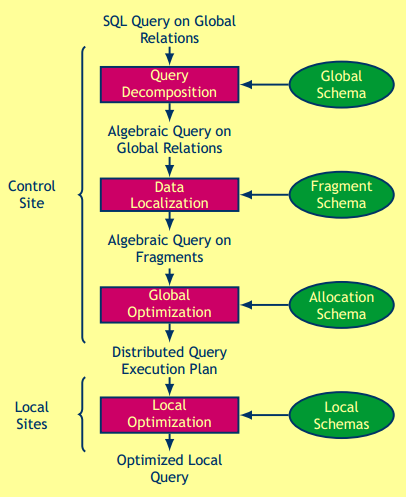
\includegraphics[scale=0.7]{src/verteilte_anfrageverarbeitung.png}\\
Zwei Schritte, um ein Query in einem verteilten System zu verarbeiten:
\begin{itemize}
\item Zerlegung
\begin{itemize}
\item Normalisierung (Bedingung in WHERE Klausel)
\item Analyse, um inkorrekte Queries zurückzuweisen
\item Vereinfachung, Redundanz beseitigen
\item Umformen in optimalen Ausdruck der relationalen Algebra
\end{itemize}
\item Lokalisierung
\begin{itemize}
\item verwenden des Fragmentierungsschema
\item vertilte Anfrage mit globalen Relationen abbilden in Anfragen mit Fragmenten
\begin{itemize}
\item Ersetzen der globalen Relation mit Fragmenten
\item $\cup$ für horizontale Fragmentierung
\item $\bowtie$ für vertikale Fragmentierung
\end{itemize}
\item optimieren der lokalisierten Anfrage durch Reduktion
\begin{itemize}
\item Reduktion mit Selektion / Join
\end{itemize}
\end{itemize}
\end{itemize}
\subsection{Reduktionen}
\subsubsection{Beispielrelationen}
% first column
\begin{minipage}[t]{0.45\textwidth}
AUF(ANr, Datum, KNr) ist fragmentiert:\\
AUF1 = $\sigma_{ANr \leq A3}$(AUF)\\
AUF2 = $\sigma_{A3<ANr \leq A6}$(AUF)\\
AUF3 = $\sigma_{ANr>A6}$(AUF)\\
AUF = AUF1 $\cup$ AUF2 $\cup$ AUF3\\
\\
APOSTEN(ANr, BNr, Menge) ist fragmentiert:\\
APO1 = $\sigma_{ANr \leq A3}$(APO)\\
APO2 = $\sigma_{ANr>A3}$(APO)\\
APO = APO1 $\cup$ APO2\\
\\
KUNDEN(KNr, KName, Ort) ist fragmentiert:\\
KUN1 = $\pi_{KNr,KName}$(KUN)\\
KUN2 = $\pi_{KNr,Ort}$(KUN)\\
KUN = KUN1 $\bowtie$ KUN2\\
\end{minipage}
\hspace{0.1\textwidth}
%second column
\begin{minipage}[t]{0.45\textwidth}
Für Reduktion in DHF:\\
KUNDEN(KNr, KName, Ort) ist fragmentiert:\\
KUN1 = $\sigma_{Ort=Basel}$(KUN)\\
KUN2 = $\sigma_{Ort \neq Basel}$(KUN)\\
KUN = KUN1 $\cup$ KUN2\\
\\
AUFRAEGE(ANr, Datum, KNr) ist abgeleitet fragmentiert:\\
AUF1 = AUF $\ltimes$ KUN1\\
AUF2 = AUF $\ltimes$ KUN2\\
AUF = AUF1 $\cup$ AUF2
\end{minipage}
\subsubsection{PHF mit Selektion}
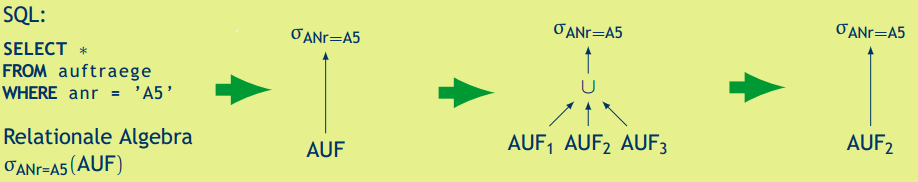
\includegraphics[scale=0.7]{src/phf_select.png}
\subsubsection{PHF mit Join}
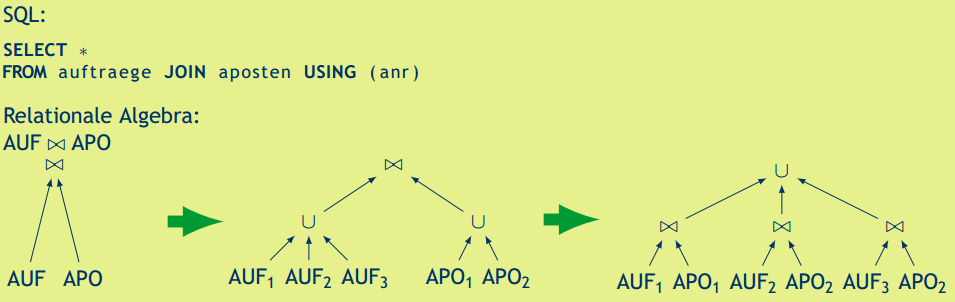
\includegraphics[scale=0.7]{src/phf_join.png}
\subsubsection{VF}
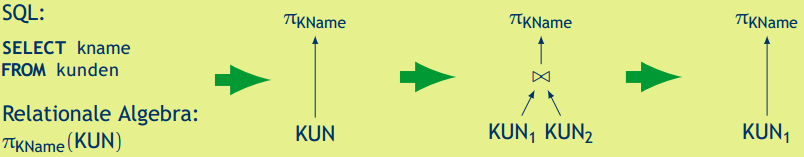
\includegraphics[scale=0.7]{src/vf.png}
\subsubsection{DHF}
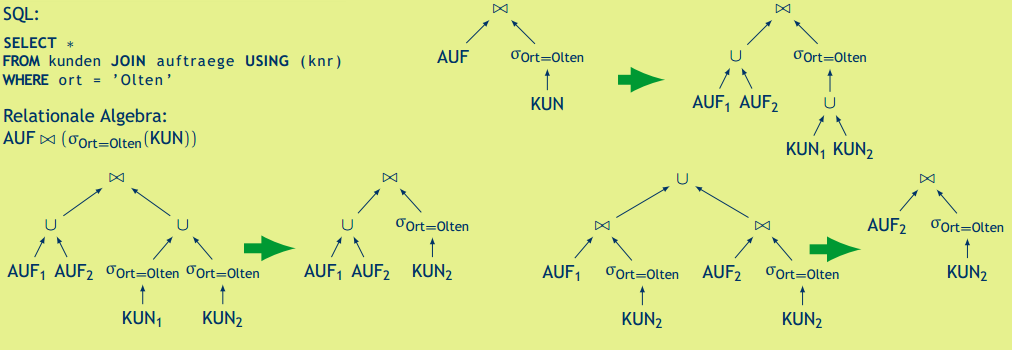
\includegraphics[scale=0.65]{src/dhf_red.png}
\subsection{SemiJoin}
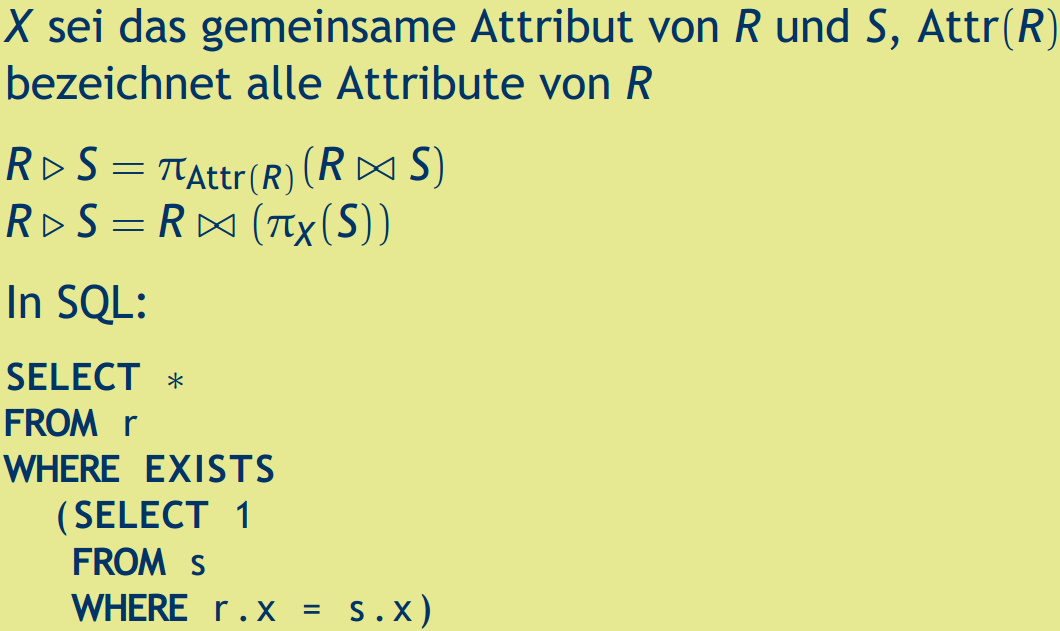
\includegraphics[width=15cm]{src/semijoin.png}\\
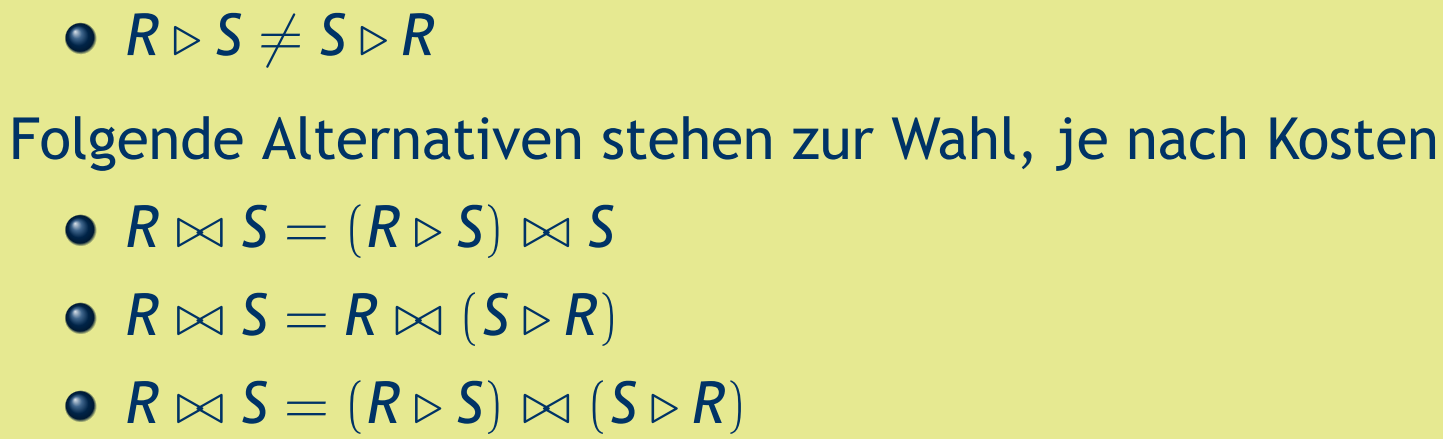
\includegraphics[width=15cm]{src/semijoin2.png}\\
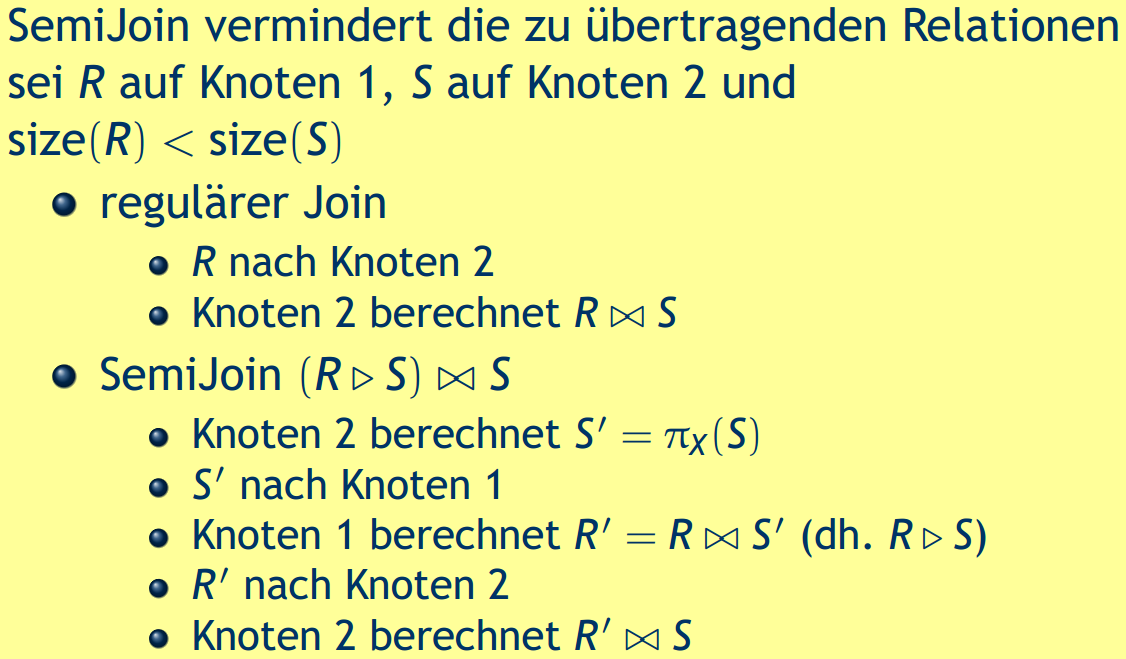
\includegraphics[width=15cm]{src/semijoin3.png}
\section{Kapitel 5 - Distributed Transactions I}
\section{Kapitel 6 - Distributed Transactions II}
\section{Kapitel 7 - Replication I}
\section{Kapitel 8 - Replication II}
\section{Kapitel 9 - NoSQL}
\section{Kapitel 10 - Cassandra}
\section{Kapitel 11 - MapReduce}
\section{Kapitel 12 - mongoDB}
\section{Kapitel 13 - Neo4j}
\section{Kapitel 14 - Semantic Web}
\end{document}
